\section{Priors}
\paragraph*{Prior.} The term $p(\theta)$ is called prior distribution. It describes the uncertainty about the model parameter $\theta$ before observing (additional) data. So, it reflects our level of ignorance. Determining the prior is the most vodoo-part in the Bayesian approach. Infact it is the main point of criticism. Often one uses uninformative priors, (which are not necessarily uniform priors) or/and priors that are conjugate to a given likelihood function.
More details may be found in Ref. \cite{robert}, Chap. 3.
\subsection{Conjugate priors}
\begin{definition}[Conjugacy\cite{robert}] A family of $\mathcal F$ of probability distributions on $\Theta$ is called conjugate to a likelihood function $f(x|\theta) :\Leftrightarrow$  $\forall \pi \in \mathcal F$ the posterior distribution $\pi(\theta|x) \in \mathcal F$.  
\end{definition}
It is known that for the exponential family there always exists a conjugate prior. Furthermore conjugate priors are quite well studied.
Let's summarize the relevant ones for us in Table \ref{tab:conjugate_priors}.
\begin{table}
\begin{tabular}{lll}
\hline \hline
Likelihood & Prior &Posterior \\
$pk(x|\theta)$ & $\pi(\theta)$ & $\pi(\theta|x)$ \\
\hline
$ Bin (n, \theta)$ &  $Beta (\alpha, \beta)$ &  $Beta (\alpha +x, \beta + n -x)$  \\
$Mult_k(\theta_1 \dots \theta_k, n)$ 
& $Dir_k(\alpha_1 \dots \alpha_k)$   
& $Dir_k(\alpha_1 + x_1 \dots \alpha_k + x_k)$  \\
\hline\hline
\end{tabular}
\caption{\label{tab:conjugate_priors}Conjugate priors for given likelihoods.}
\end{table}
\paragraph*{Example: Conjugate Prior for the Binomial distribution.} This example shows that the Beta distribution is the conjugate prior to the binomial distribution. Assume the model for the data is $P(X|\theta)=Bin(x|\theta, n)$ ($\theta$ is the success probability and $n$ is the number of trials) and chose the Beta distribution as Prior, $P(\theta) = Beta(\theta|\alpha, \beta) $. Then we get as posterior
\begin{align} \label{eq:beta_binom}
p(\theta |x, n, \alpha, \beta) &=\frac{1}{N} Bin(x|n,\theta) Beta(\theta|\alpha, \beta) \\
& = \frac{1}{N}  \frac{\binom {n} {x} \theta^{x + \alpha-1} (1-\theta)^{n-x+\beta -1}}{B(\alpha, \beta)}  \\
& = Beta(\theta | x + \alpha, n-x+\beta),
\end{align} 
again a Beta distribution with updated parameters. The factor $1/N$ is just the normalization constant, which may be obtained be integrating the right hand side over $\theta$. The normalization requirement leads to the general trick to only consider the functional form of the free variables (in this case $\theta$) and identify the posterior distribution only via the functional form. The rest is done by the normalization requirement. For this example we would have
\begin{align}
 p(\theta |x, n, \alpha, \beta) &\propto Bin(x|n,\theta) Beta(\theta|\alpha, \beta) \\ 
 &\propto \theta^{x + \alpha-1} (1-\theta)^{n-x+\beta -1} \\ 
 &\propto Beta(\theta | x + \alpha, n-x+\beta)
\end{align}

In order to clarify how the conditionals in the first line emerge it's instructive to look at the joint distribution,
\begin{align*}
p(\theta, \alpha, \beta, n, x) = p(x|\theta, n) p(\theta|\alpha, \beta) p(n) p(\alpha) p(\beta)
\end{align*}
\begin{figure}
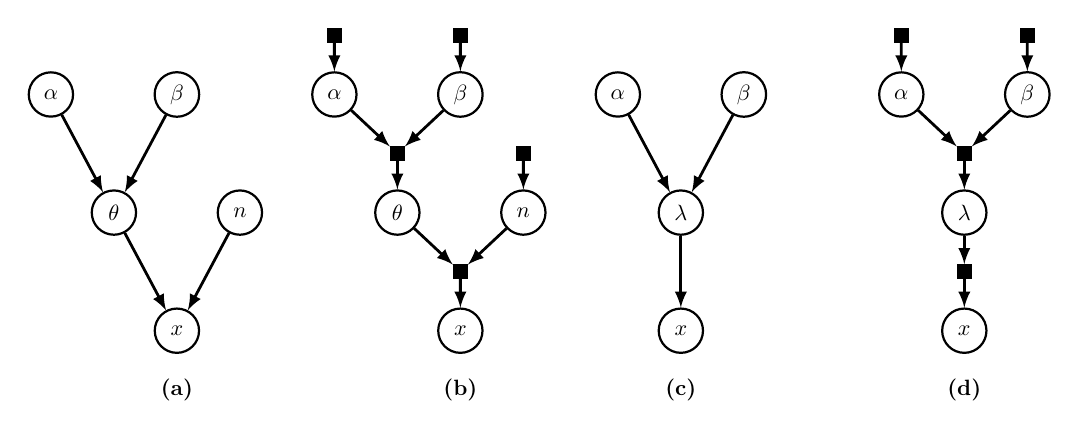
\begin{tikzpicture}[thick,xscale=0.8, yscale=.75, every node/.style={scale=0.8}]
\tikzset{vertex/.style = {shape=circle,draw,minimum size=2em}}
\tikzset{edge/.style = {->,> = latex, line width=1}}

% binomial beta directed graph
\begin{scope}
% vertices
\node[vertex] (a) at  (-1,2) {$\alpha$};
\node[vertex] (b) at  (1,2) {$\beta$};
\node[vertex] (x) at  (1, -2) {$x$};
\node[vertex] (n) at (2,0) {$n$};
\node[vertex] (t) at (0,0) {$\theta$};
%edges
\draw[edge] (a) to (t);
\draw[edge] (b) to (t);
\draw[edge] (t) to (x);
\draw[edge] (n) to (x);
\node at (1, -3) {\textbf{(a)}}; 
\end{scope}

% binomial beta factor graph
\begin{scope}[shift={(4.5,0)}]
% vertices
\node[vertex] (a) at  (-1,2) {$\alpha$};
\node[vertex] (b) at  (1,2) {$\beta$};
\node[vertex] (x) at  (1, -2) {$x$};
\node[vertex] (n) at (2,0) {$n$};
\node[vertex] (t) at (0,0) {$\theta$};
\begin{scope}[vertex/.style = {shape=rectangle, draw,minimum size=.1em, inner sep=3pt, fill=black}]
\node[vertex] (fone) at  (-1,3) {};
\node[vertex] (ftwo) at  (1,3) {};
\node[vertex] (fthree) at (0,1) {};
\node[vertex] (ffour) at (1,-1) {};
\node[vertex] (ffife) at (2,1) {};
\end{scope}
%edges

\draw[edge] (fone) to (a);
\draw[edge] (ftwo) to (b);
\draw[edge] (a) to (fthree);
\draw[edge] (b) to (fthree);
\draw[edge] (fthree) to (t);
\draw[edge] (t) to (ffour);
\draw[edge] (n) to (ffour);
\draw[edge] (ffour) to (x);
\draw[edge] (ffife) to (n);
\node at (1, -3) {\textbf{(b)}}; 
\end{scope}

% poisson gamma directed graph
\begin{scope}[shift={(9,0)}]
% vertices
\node[vertex] (a) at  (-1,2) {$\alpha$};
\node[vertex] (b) at  (1,2) {$\beta$};
\node[vertex] (l) at (0,0) {$\lambda$};
\node[vertex] (x) at (0,-2) {$x$};
%edges
\draw[edge] (a) to (l);
\draw[edge] (b) to (l);
\draw[edge] (l) to (x);
\node at (0, -3) {\textbf{(c)}}; 
\end{scope}

% poisson gamma factor graph
\begin{scope}[shift={(13.5,0)}]
% vertices
\node[vertex] (a) at  (-1,2) {$\alpha$};
\node[vertex] (b) at  (1,2) {$\beta$};
\node[vertex] (l) at (0,0) {$\lambda$};
\node[vertex] (x) at (0,-2) {$x$};
\begin{scope}[vertex/.style = {shape=rectangle, draw,minimum size=.1em, inner sep=3pt, fill=black}]
\node[vertex] (f1) at  (-1,3) {};
\node[vertex] (f2) at  (1,3) {};
\node[vertex] (f3) at  (0,1) {};
\node[vertex] (f4) at  (0,-1) {};
\end{scope}
%edges
\draw[edge] (f1) to (a);
\draw[edge] (f2) to (b);
\draw[edge] (a) to (f3);
\draw[edge] (b) to (f3);
\draw[edge] (f3) to (l);
\draw[edge] (l) to (f4);
\draw[edge] (f4) to (x);
\node at (0, -3) {\textbf{(d)}}; 
\end{scope}

\end{tikzpicture}


\caption{\label{fig:graphs_for_conj_priors}Directed graph (a) and factor graph (b) for beta distribution as conjugate prior of the binomial distribution. (c) and (d) shows the directed and factor graph for the Gamma distribution as conjugate prior of the Poisson distribution.}
\end{figure}
The structure of the underlying model is more transparent in a graph representation (Fig.\,\ref{fig:graphs_for_conj_priors} (a) and (b)). Apart from the Beta and Binomial distributions, there are the additional terms from the individual parameters. These terms eventually cancel in the computation for the conditional distribution,
\begin{align*}
p(\theta | \alpha, \beta, n, x)  &= \frac{p(\theta, \alpha, \beta, n, x)}{p(\alpha, \beta, n, x)} = \frac{p(\theta, \alpha, \beta, n, x)}{\int p(\theta, \alpha, \beta, n, x)\,d\theta} \\ &= \frac{p(x|n, \theta) p(\theta|\alpha, \beta)}{\int p(x|\theta, n) p(\theta|\alpha, \beta) \,d\theta},
\end{align*} 
which is just Equation \ref{eq:beta_binom} with the explicit form of the normalization constant.
\paragraph*{Example: Conjugate Prior for the Poisson distribution.} This example shows that the Gamma distribution is the conjugate prior to the Possion distribution. Assume the model for the data is a Poisson distribution,
\begin{align}
p(x|\lambda)= \frac{\lambda^x e^{-\lambda}}{x!},
\end{align}   
with $x$ number of counts. Chose the Gamma distribution $\Gamma(\lambda|\alpha, \beta)$  as Prior and assume only one Poisson experiment $x=(x)$ (see Fig.\,\ref{fig:graphs_for_conj_priors (c) and (d)}. Then we get as posterior
\begin{align}
p(\lambda|x, \alpha, \beta)  
&\propto  \frac{\lambda^x e^{-\lambda}}{x!} \Gamma(\lambda|\alpha, \beta) \\
&\propto \lambda^{(\alpha + x) - 1} e^{-\lambda(\beta +1)} \\
&\propto \Gamma(\lambda | \alpha + x, \beta +1)
\end{align} 
So, for one experiment $\alpha$ is updated by the number of counts  $x$  and $\beta$ is updated by the number of experiments (which is one). 

Now let's consider the case where we perform $n$ IID Poisson experiments, $x=(x_1, \dots, x_n)$. \textbf{(TODO graph with plate notation)} Then the likelihood becomes
\begin{align}
p(x|\lambda)= \prod _{i=1} ^n \frac{\lambda^{x_i} e^{-\lambda}}{x_i!}
=  \frac{\lambda^{\sum_{i=1}^n x_i} e^{-n \lambda}}{\prod _{i=1} ^n x_i!}
\end{align}
Then the posterior is obtained by
\begin{align}
p(\lambda|x, \alpha, \beta)  
&\propto  \frac{\lambda^x e^{-\lambda}}{x!} \Gamma(\lambda|\alpha, \beta) \\
&\propto  \lambda^{(\alpha + \sum_{i=1}^n x_i) - 1} e ^ {\lambda (\beta + n)} \\
&\propto \Gamma(\lambda | \alpha + \sum_{i=1}^n x_i, \beta +n)
\end{align}
So, for $n$ Poisson experiments the $\alpha$ parameter of the Gamma distribution is updated by the total number of counts (of all experiments) and beta is updated by the number of experiments ($n$ in this case).
\begin{theorem}
There exist conjugate priors for the exponential family of distributions.
\end{theorem}
